\appendix
\chapter{Appendix}

Following Table \ref{Evaluation losses of the differences comparison between architectures and Transformer blocks} as well as Figure \ref{Super-resolution images from the DP-TF Transformer and SwinIR+DP models} and \ref{Super-resolution images from the conditions subsequently as true} show the evaluation of the difference mentioned in the section
\ref{comparison between the architecture}.

\begin{table}[!htp]
    \centering
    \caption{Evaluation losses of the differences between architectures and Transformer blocks}
    \label{Evaluation losses of the differences comparison between architectures and Transformer blocks}
    \begin{tabular}{l|c|c|c|c|c|c}
        \hline
        Transformer difference & \#Params & MSE & SDR & LSD & WMSE & Perceptual \\
        \hline
        DP & 48,042 & 1.731 & -5.375 & 0.380 & 0.179 & 12.320\\
        \hline
        SwinIR+DP & 30,562 & 1.662 & -6.415 & 0.360 & 0.128 & 16.903 \\
        \hline
        Condition1 & 84,258 & 1.562 & -5.784 & 0.372 & 0.155 & 12.866 \\
        \hline
        Condition2 & 84,130 & 1.490 & -5.367 & 0.380 & 0.363 & 13.102 \\
        \hline
        Condition3 & 47,074 & 1.779 & -5.333 & 0.382 & 0.176 & 13.343 \\
        \hline
        Condition4 & 47,074 & 1.364 & -4.986 & 0.388 & 0.170 & 13.436 \\
        \hline
        Condition5 & 42,786 & 1.671 & -5.215 & 0.384 & 0.164 & 14.410 \\
        \hline
        Condition6 & 34,466 & 2.040 & -5.181 & 0.387 & 0.206 & 15.945 \\
        \hline
        Condition7 & 30,178 & 4.415 & -5.718 & 0.377 & 0.272 & 17.011 \\
        \hline
        Condition8 & 30,178 & 1.435 & -6.523 & 0.359 & 0.150 & 15.112 \\
        \hline
        Condition9 & 30,178 & 1.568 & -5.805 & 0.373 & 0.166 & 14.807 \\
        \hline
        Condition10 & 30.178 & 2.026 & -5.980 & 0.369 & 0.169 & 15.887 \\
        \hline
        Condition11 & 30.178 & 5.004 & -7.837 & 0.338 & 0.256 & 20.567 \\
        \hline
        Condition12 & 30.178 & 3.474 & -7.513 & 0.343 & 0.265 & 19.121 \\
        \hline
    \end{tabular}
\end{table}


\begin{figure}[t]
    \centering
    \begin{subfigure}{0.95\textwidth}
        \centering
        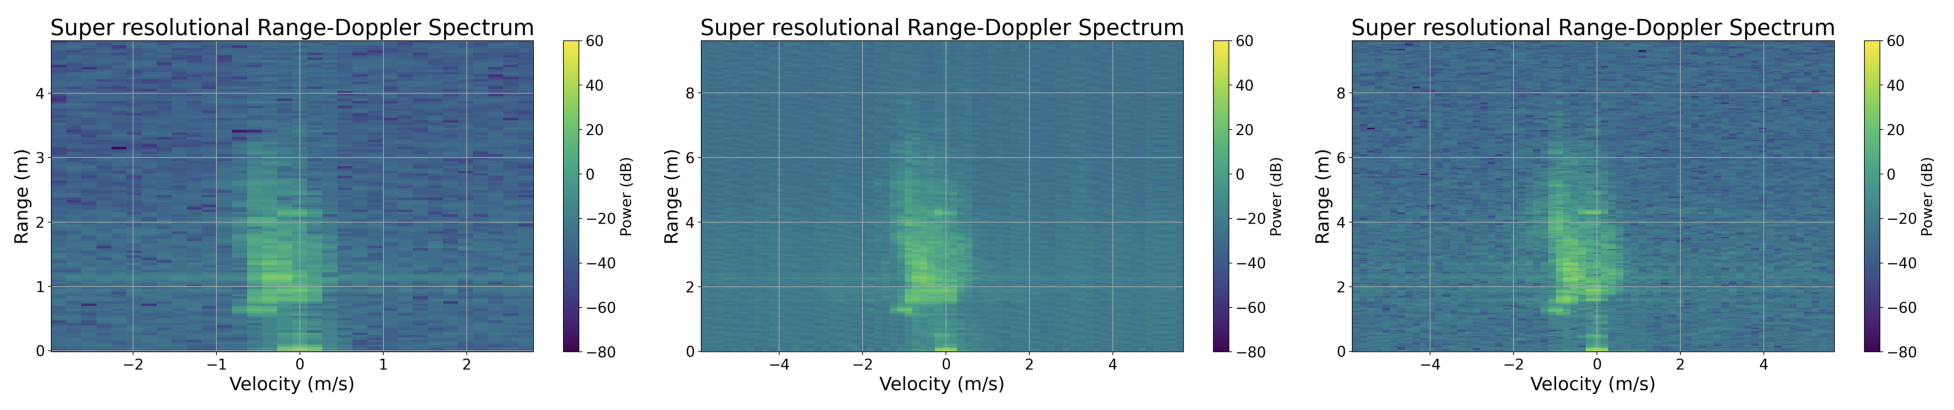
\includegraphics[width=\textwidth]{thesis/figures/evaluation_difference_0.png}
        \caption{Super-resolution range-Doppler map from the DP-TF Transformer model}
        \label{Super-resolution image from the DP-TF Transformer model}
    \end{subfigure}
    \vspace{0.3cm}
    \begin{subfigure}{0.95\textwidth}
        \centering
        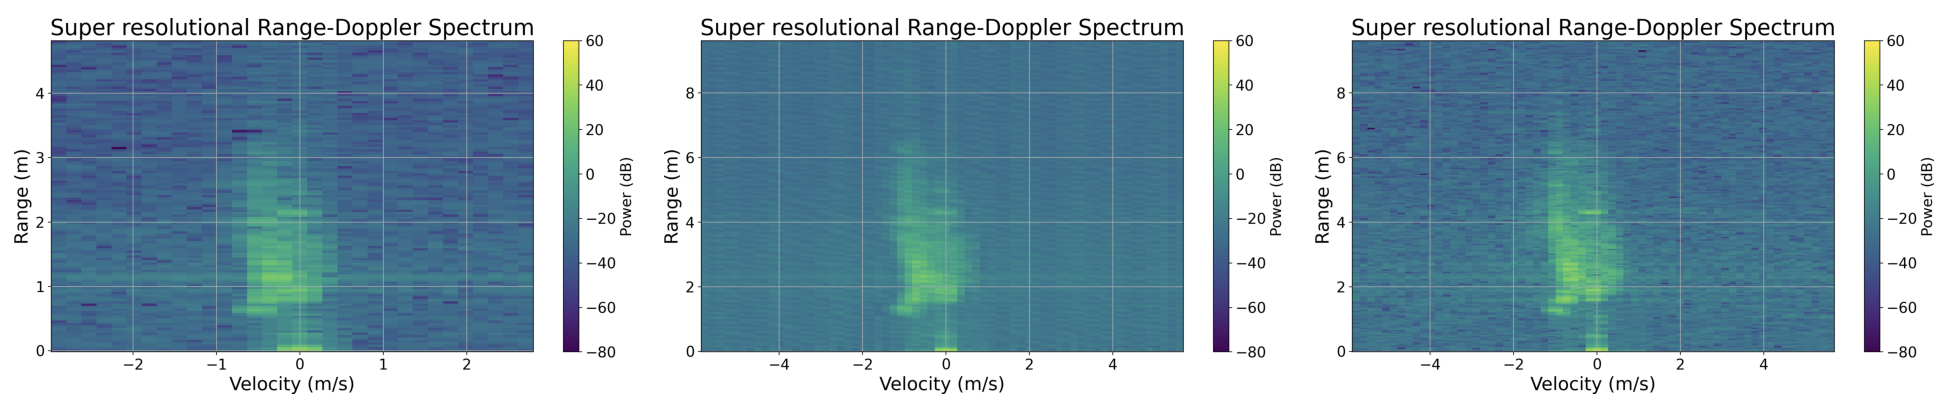
\includegraphics[width=\textwidth]{thesis/figures/evaluation_difference_0+.png}
        \caption{Super-resolution range-Doppler map from the SwinIR+DP model}
        \label{Super-resolution image from the SwinIR+DP model}
    \end{subfigure}
    \caption{Super-resolution range-Doppler maps from both models}
    \label{Super-resolution images from the DP-TF Transformer and SwinIR+DP models}
\end{figure}

\begin{figure}[t]
    \centering
    \begin{subfigure}{0.95\textwidth}
        \centering
        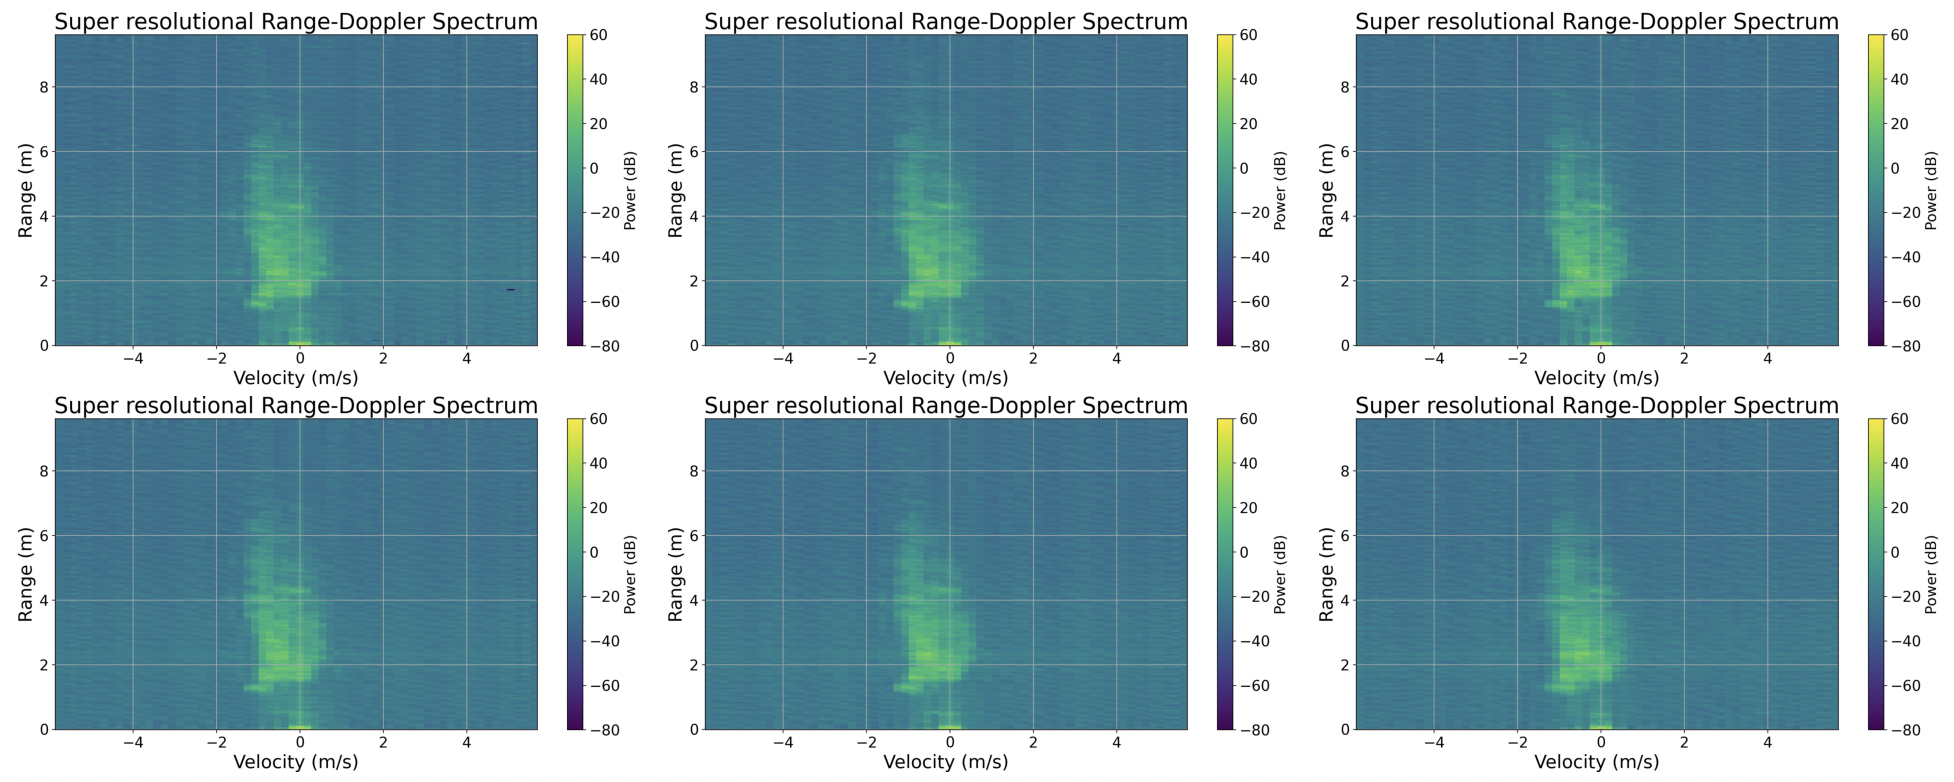
\includegraphics[width=\textwidth]{thesis/figures/evaluation_difference_1-6.png}
        \caption{Super-resolution range-Doppler maps as the condition 1 - 6 subsequently as true}
        \label{Super-resolution images from the condition 1 to condition 6 subsequently as true}
    \end{subfigure}
    \vspace{0.3cm}
    \begin{subfigure}{0.95\textwidth}
        \centering
        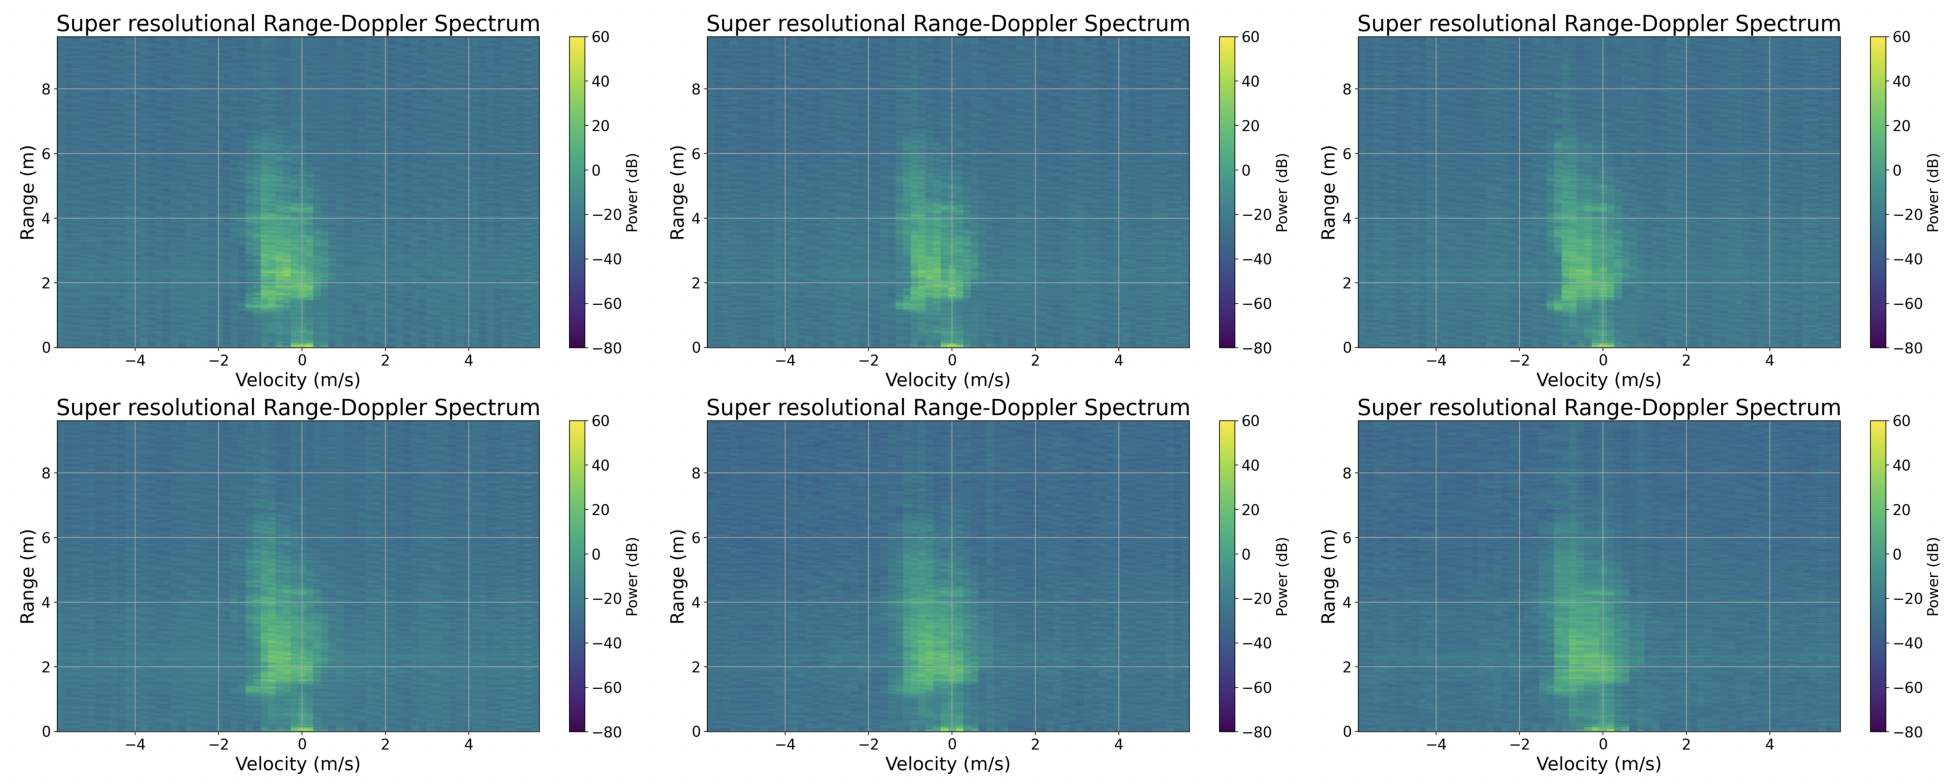
\includegraphics[width=\textwidth]{thesis/figures/evaluation_difference_7-12.png}
        \caption{Super-resolution range-Doppler maps as the condition 7 - 12 subsequently as true}
        \label{Super-resolution images from the SwinIR+DP model}
    \end{subfigure}
    \caption{Super-resolution range-Doppler maps from the conditions subsequently as true}
    \label{Super-resolution images from the conditions subsequently as true}
\end{figure}